%!TEX root = project.tex

\chapter*{About this project}
\paragraph{Abstract}
The 3D game engine Unity provides a great framework for any novice game developer, even experienced developers and studios use this engine as a bases for their AAA games. For these reasons, I have chosen to use the Unity 3D engine as the essential framework for this mobile 3D game. The game's development has been contracted by Pat McNeill at the company Agmanor. I found that game development is much more complicated then I previously expected. For instance the assets require like models, textures, level design, gameplay scripting, player progression, environment, the jobs to complete seemly never end on this project. The original concept of the game was vague, it was described to be farming game that required the player to buy and sell cattle, and eventually grow your farm into a profitable enterprise. The project's artwork, UI interface and storyline, essential items basically, were left out during the initial designing phase, which later turned out to be some of the more challenging aspects in development phase of the project. Unity's 3D game engine 

\paragraph{Authors}
The authors of this document; John Walsh, B.Sc. Ordinary Degree - GMIT

\chapter{Introduction}
The 3D gaming world has evolved immensely over the last few years. More gamers are looking to new devices like the mobile platform whether it be an Android and iOS device. This presents new challenges for game develops to not only target multiple platforms, but also deliver a well refined, complex and engaging story lines with high resolution textures and models. This problem is further compounded when developers only have access to limited resources these small devices provide. Later I'll discuss some of these problems faced in design and development of this 3D mobile game project. 
   
\section{Context}
The game world will be constructed in 3D open environment, which means the player will be able to freely navigate their way around the world. A virtual joystick has been implemented to allow users use the touchscreen feature on their device to control the character[~\cite{einstein}]. The main camera view will be locked into an isometric angle giving the user a third person view of the character. From this point of view the player will be able to see most of the environment and intractable game objects around the character. User's interact with the game's menu system primarily by touch. Frameworks like NGUI have been employed to help scale and display the menu's elements in a consistent design. Transitions between levels will be handled when the player’s character comes into contact with a special object / area in-game that triggers an event to display a menu. This menu allows the player to transition from either the farm scene to the mart scene or back to the main menu. Target audiences for this game could roughly range from 6 + or older, I'm not entirely certain what age group this game fits into. I believe the game has potential to grow and develop into more than just another farm simulator game. From an education point of view the game could be modified to teach kids more about farm animals and how to properly look after the animals.

\section{Objectives}
The first objective of the project was to design an application that would satisfy both the client and gamers when fully released to the market. During initial few weeks of development, I had to up skill on the different tools available in the Unity IDE editor. Since the requires an open environment, tools like the terrain editor, transform position component and assets required to fill the game scene were experimented with heavily during the initial versions of the game. 
After some time getting acquainted with the development tools, it was at this stage I needed to source proper assets that would fit with the theme, artwork and gameplay features. The developers of Unity 3D have constructed an assets store that contains some useful materials and tools that greatly decrease the development time required to construct scene levels and game objects.
\section{Chapters Review}
In this chapter I'll be briefly reviewing the different areas of this paper. From the design and planning phase to the implementation phase.
\subsection{Methodology}
In this chapter I'll cover the different development tools and practices I've used during the implementation phase of the project. Work on the project has been recorded and documented using the tool collaboration GitHub, I believe it would be prudent to review commits in project repository[~\cite{einstein}]
\begin{itemize}
	\item Provide a context for your project.
	\item Set out the objectives of the project
	\item Briefly list each chapter / section and provide a 1-2 line description of what each section contains.
	\item List the resource URL (GitHub address) for the project and provide a brief list of the main elements at the URL.
\end{itemize}

\subsection{Technology Review}
The different technologies used to design and implement the project from start to finish. Everything from the tools used to the software development approaches employed to create an efficient and effective foundation for the game to be built upon.
\subsection{System Design}
System design will cover the different modules and classes implemented to perform a particular function whether it be gameplay scripting to UI implementation.
\subsection{Conclusion}
Final conclusion from the overall design and development of the project, I will review the final product and discuss different parts of the implementation that could've been developed differently, maybe even more efficiently then the current version of the project.
\section{Resources}

Make sure you use references~\cite{einstein}

\chapter{Methodology}
About one to two pages.
Describe the way you went about your project:
\begin{itemize}
\item Agile / incremental and iterative approach to development. Planning, meetings.
\item What about validation and testing? Junit or some other framework.
\item If team based, did you use GitHub during the development process.
\item Selection criteria for algorithms, languages, platforms and technolo-gies.
\end{itemize}
Check out the nice graphs in Figure \ref{tikz:graphs}, and the nice diagram in Figure \ref{tikz:mydiagram}.

\begin{figure}
  \centering
  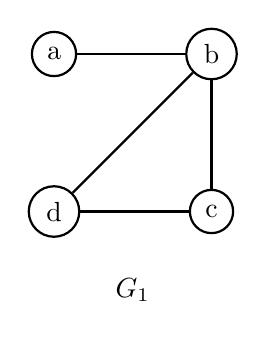
\begin{tikzpicture}
  \begin{scope}[every node/.style={circle,thick,draw}]
  \node (a) at (0,2) {a};
  \node (b) at (2,2) {b};
  \node (c) at (2,0) {c};
  \node (d) at (0,0) {d};
  \end{scope}
  \begin{scope}[every edge/.style={draw=black,thick}]
  \path (a) edge (b);
  \path (b) edge (c);
  \path (b) edge (d);
  \path (c) edge (d);
  \end{scope}
  \node () at (1,-1) {$G_1$};
  \end{tikzpicture}
  \hspace{1.5cm}
  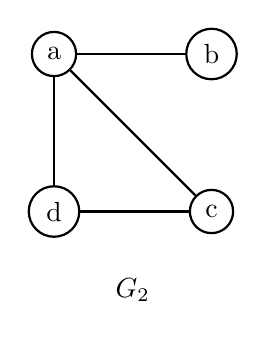
\begin{tikzpicture}
  \begin{scope}[every node/.style={circle,thick,draw}]
  \node (1) at (0,2) {a};
  \node (2) at (2,2) {b};
  \node (3) at (2,0) {c};
  \node (4) at (0,0) {d};
  \end{scope}
  \begin{scope}[every edge/.style={draw=black,thick}]
  \path (1) edge (2);
  \path (1) edge (3);
  \path (1) edge (4);
  \path (3) edge (4);
  \end{scope}
  \node () at (1,-1) {$G_2$};
  \end{tikzpicture}
  \caption{Nice pictures}
  \label{tikz:graphs}
\end{figure}

\begin{figure}
  \centering
  \begin{tikzpicture}[node distance=6cm]
  \node (a) [rect] {A Big Blue Block};
  \node (b) [oval, right of=a] {And His Oval Friend};
  \draw [line] (a) -- (b);
  \end{tikzpicture}
  \caption{Nice pictures}
  \label{tikz:graphs}
\end{figure}

\chapter{Technology Review}
About seven to ten pages.
\begin{itemize}
\item Describe each of the technologies you used at a conceptual level. Standards, Database Model (e.g. MongoDB, CouchDB), XMl, WSDL, JSON, JAXP.
\item Use references (IEEE format, e.g. [1]), Books, Papers, URLs (timestamp) – sources should be authoritative. 
\end{itemize}

\section{XML}
Here's some nicely formatted XML:
\begin{minted}{xml}
<this>
  <looks lookswhat="good">
    Good
  </looks>
</this>
\end{minted}

\chapter{System Design}
As many pages as needed.
\begin{itemize}
\item Architecture, UML etc. An overview of the different components of the system. Diagrams etc… Screen shots etc.
\end{itemize}

\begin{table}[h]
  \centering
  \begin{tabular}{x{2cm}p{3cm}}
    \toprule \\
    Column 1 & Column 2 \\
    \midrule \\
    Rows 2.1 & Row 2.2 \\
    \bottomrule
  \end{tabular}
  \caption{A table.}
  \label{table:mytable}
\end{table}

\chapter{System Evaluation}
As many pages as needed.
\begin{itemize}
\item Prove that your software is robust. How? Testing etc. 
\item Use performance benchmarks (space and time) if algorithmic.
\item Measure the outcomes / outputs of your system / software against the objectives from the Introduction.
\item Highlight any limitations or opportuni-ties in your approach or technologies used.
\end{itemize}

\chapter{Conclusion}
About three pages.

\begin{itemize}
\item Briefly summarise your context and ob-jectives (a few lines).
\item Highlight your findings from the evalua-tion section / chapter and any opportuni-ties identified.
\end{itemize}

